\documentclass[a4paper]{article}
\usepackage[14pt]{extsizes} 
\usepackage[T2A]{fontenc}
\usepackage[utf8]{inputenc}
\usepackage{natbib}
\usepackage{graphicx}
\usepackage{amsmath}
\usepackage[english, russian]{babel}
\usepackage{amsmath,amsfonts,amssymb,amsthm,mathtools,mathrsfs}
\usepackage{icomma}
\usepackage{fullpage}
\usepackage{ulem}
\usepackage{eufrak}
\usepackage{setspace}
\usepackage{listings}
\usepackage{indentfirst}
\usepackage[left=2cm,right=1.5cm,top=2cm,bottom=2cm]{geometry}
\usepackage{xcolor}
\usepackage{float}
\usepackage{csquotes}

\setlength{\parindent}{5ex}
\setlength{\parskip}{1em}
\renewcommand{\baselinestretch}{1}

\graphicspath{{images/}}

\definecolor{buzzlightyear}{HTML}{8757A5}
\definecolor{grass}{HTML}{738D06}
\definecolor{literal}{HTML}{F18A2B}
\definecolor{commentcolor}{HTML}{8E908B}

\lstdefinestyle{habrstyle}{
    backgroundcolor=\color{white},   
    commentstyle=\color{commentcolor},
    keywordstyle=\bfseries\color{buzzlightyear},
    numberstyle=\tiny\color{commentcolor},
    stringstyle=\color{grass},
    basicstyle=\ttfamily\footnotesize,
    breakatwhitespace=false,         
    breaklines=true,                 
    captionpos=b,                    
    keepspaces=true,                 
    numbers=left,                    
    numbersep=5pt,                  
    showspaces=false,                
    showstringspaces=false,
    showtabs=false,                  
    tabsize=4
}

\lstset{style=habrstyle}

\begin{document}
    % НАЧАЛО ТИТУЛЬНОГО ЛИСТА
    \begin{center}
        \begin{center}
        \hfill \break
        \normalsize{Санкт-Петербургский государственный политехнический}\\
        \normalsize{университет Петра Великого}\\
        \hfill \break
        \normalsize{\textbf{Высшая школа интеллектуальных систем и}}\\ 
        \normalsize{\textbf{суперкомпьютерных технологий}}\\ 
        \hfill \break
        \hfill \break
        \hfill \break
        \normalsize{Лабораторная работа №1}\\
        \hfill \break
        \hfill \break
        \normalsize{\LARGE Сигналы и звуки}\\
        \end{center}
        \hfill \break
        \hfill \break
        \hfill \break
        \hfill \break
        \hfill \break
        \hfill \break
        \hfill \break
        \hfill \break
        \hfill \break
        \hfill \break
        \begin{flushright}
            \normalsize{Выполнил студент 3-го курса}\\
            \normalsize{группа 3530901/80201}\\
            \normalsize{Матвеец Андрей Вадимович}\\
            \hfill \break
            \normalsize{Преподаватель:}\\
            \normalsize{Богач Наталья Владимировна}\\
        \end{flushright}
        \hfill \break
        \hfill \break
        \hfill \break
        \hfill \break
        \begin{center} Санкт-Петербург\end{center}
        \begin{center}2021\end{center} 
        \thispagestyle{empty}
    \end{center}
    % КОНЕЦ ТИТУЛЬНОГО ЛИСТА
    
    % ОГЛАВЛЕНИЕ
    \newpage
        \tableofcontents
    
    % СПИСОК ИЛЛЮСТРАЦИЙ
    \newpage
         \listoffigures
    
    % СПИСОК ЛИСТИНГОВ     
    \newpage
         \lstlistoflistings   
     
    \newpage
        \section{Часть №1: Проверка}
        
            В первом пункте данной лабораторной работы нам необходимо проверить, что все листинги работают корректно. Для этого просто пройдемся по всем примерам и запустим их.
            
            \begin{figure}[h]
                \centering
                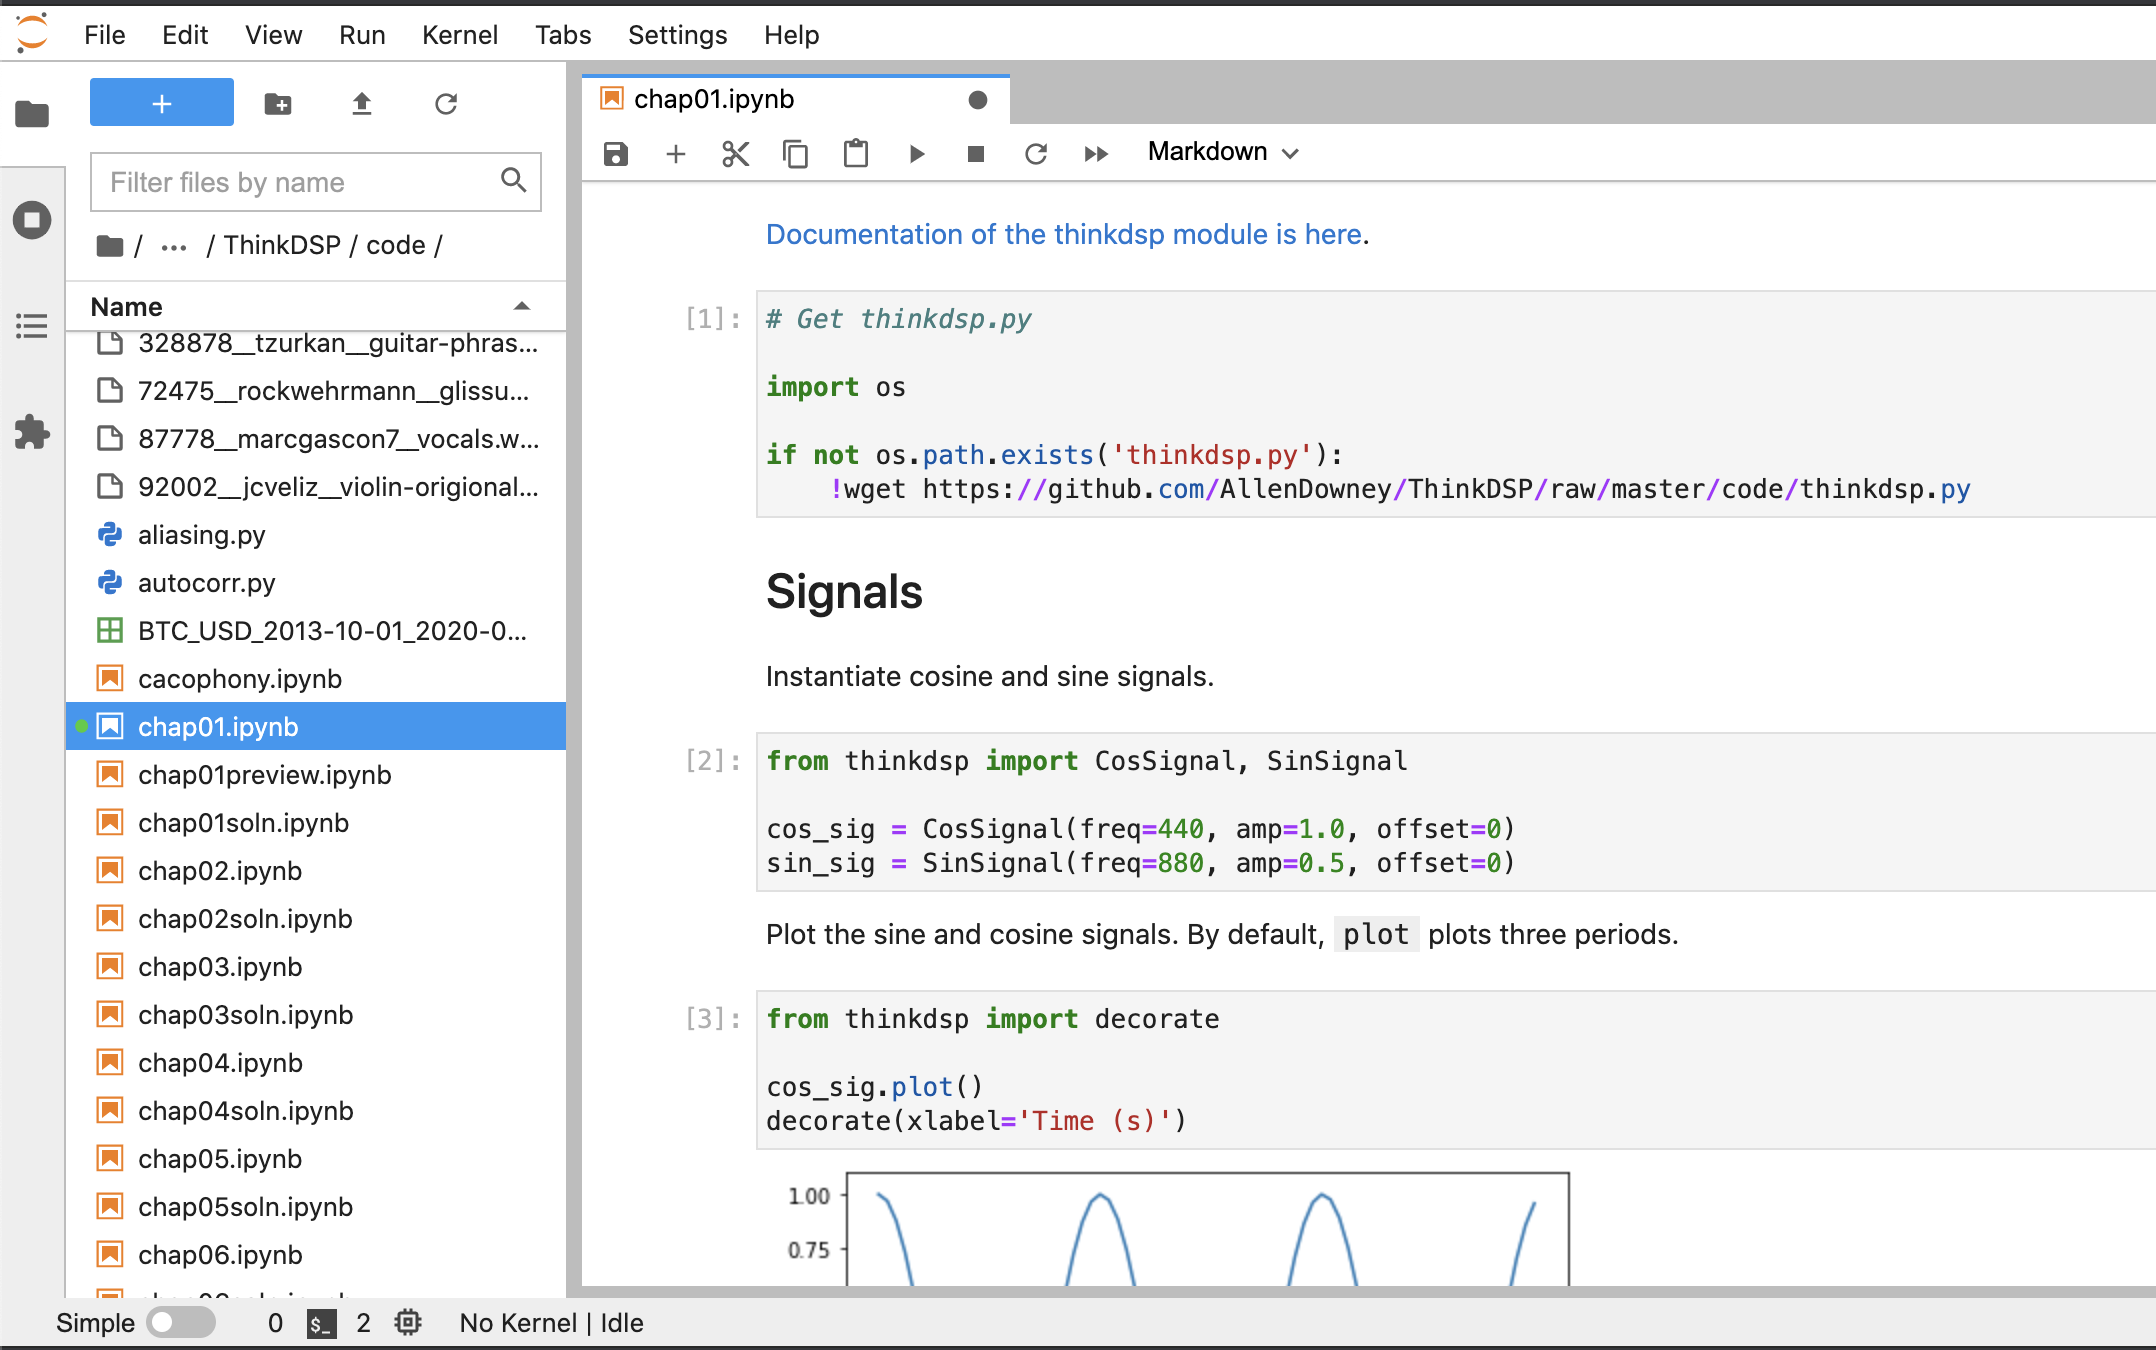
\includegraphics[width=\textwidth]{Screen_check.png}
                \caption{Проверка работоспособности}
                \label{fig:check_it_works}
            \end{figure}
            
            После прохода и запуска каждого листинга становится ясно, что все работает как ожидалось и можно переходить к следующему пункту лабораторной работы
    
    \newpage
        \section{Часть №2: Обработка}
            
            Во втором пункте первой лабораторной работы необходимо сначала скачать с сайта любой образец звука, после чего выделить в нем полсуекундный фрагмент с постоянной высотой. Необходимо вычислить и рассчитать спектр. После этого необходимо произвести фильтрацию гармоник и преобразовать спектры обратно в сигнал.
            
            Перейдем к выполнению лабораторной работы. Для начала подключим к нашему проекту \texttt{thinkdsp.py}, чтобы в дальнейшем работать с ней:
            
\begin{lstlisting}[language=Python, caption= Подключение \texttt{thinkdsp.py}]
    import os
    if not os.path.exists('thinkdsp.py'):
        !wget https://github.com/AllenDowney/ThinkDSP/raw/master/code/thinkdsp.py
\end{lstlisting}    
            
            Теперь подключим основные библиотеки, которые нам понадобятся:
            
\begin{lstlisting}[language=Python, caption= Подключение библиотек]
    from thinkdsp import read_wave
    from thinkdsp import decorate
\end{lstlisting}
        
            После этого прочтем скаченную нами ранее мелодию:
            
\begin{lstlisting}[language=Python, caption= Прочтение скаченной мелодии]
    wave = read_wave('Sounds/564668__dingeaux__shwing.wav')
    wave.normalize()
    wave.make_audio()
\end{lstlisting}
            
            После прочтения мелодии выполним \texttt{wave.plot()}: и проверим результаты вывода

\begin{lstlisting}[language=Python, caption= Просмотр \texttt{wave.plot()}]
    wave.plot()
    decorate(xlabel='Time (s)')
\end{lstlisting}

             \begin{figure}[H]
                \centering
                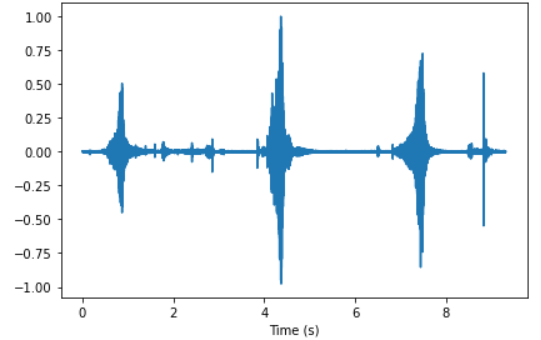
\includegraphics[width=\textwidth]{wave_plot.png}
                \caption{Результат вывода \texttt{wave.plot()}}
                \label{fig:result_output_1}
            \end{figure}
            
            Далее нам необходимо выбрать сегмент из нашей мелодии. Был выбран сегмен с 3.9 секунды и длительностью 0.5 секунды:
            
\begin{lstlisting}[language=Python, caption= Выбор сегмента]
    segment = wave.segment(start=3.9, duration=0.5)
    segment.make_audio()
\end{lstlisting}

            Теперь выведем \texttt{segment.plot()} на экран:
            
\begin{lstlisting}[language=Python, caption= Вывод \texttt{segment.plot()}]
    segment.plot()
    decorate(xlabel='Time (s)')
\end{lstlisting}
            
            \begin{figure}[H]
                \centering
                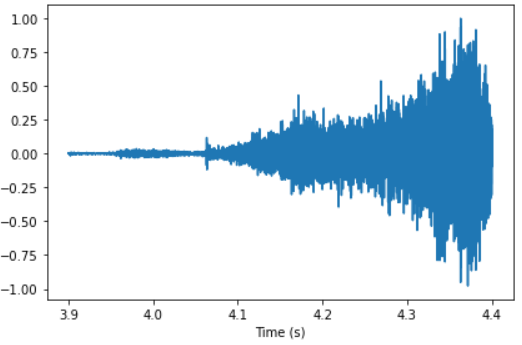
\includegraphics[width=\textwidth]{segment_plot.png}
                \caption{Результат вывода \texttt{segment.plot()}}
                \label{fig:result_output_2}
            \end{figure}
            
            После этого посмотрим как выглядит наш спектр:
            
\begin{lstlisting}[language=Python, caption= Изображение спектра]
    spectrum = segment.make_spectrum()
    spectrum.plot()
    decorate(xlabel='Frequency (Hz)')
\end{lstlisting}

            \begin{figure}[H]
                \centering
                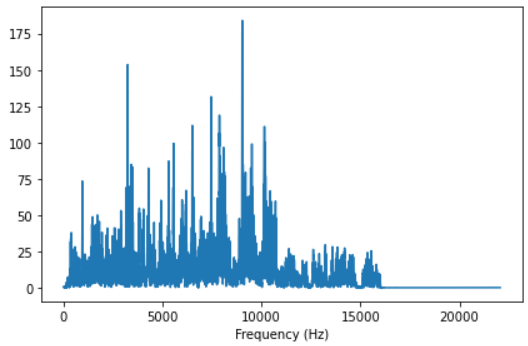
\includegraphics[width=\textwidth]{spectr_ilustr.png}
                \caption{Изображение спектра}
                \label{fig:specrt_image}
            \end{figure}
            
            Приблизим наш спектр, чтобы увидеть его более подробно:

\begin{lstlisting}[language=Python, caption= Приближенное изображение спектра]
    spectrum.plot(high=16000)
    decorate(xlabel='Frequency (Hz)')
\end{lstlisting}
            
            \begin{figure}[H]
                \centering
                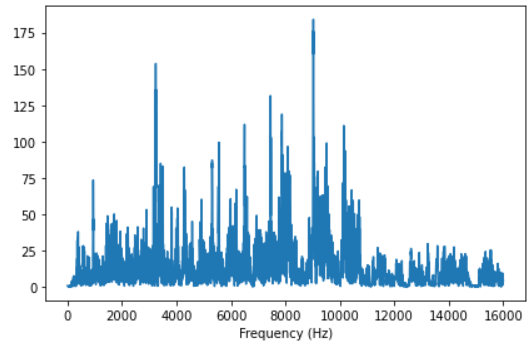
\includegraphics[width=\textwidth]{spectr_ilustr_add.png}
                \caption{Приближенное изображение спектра}
                \label{fig:spectr_image_add}
            \end{figure}
            
            Далее, полученный нам испектр необходимо отфильтровать:

\begin{lstlisting}[language=Python, caption= Фильтрация спектра]
    filtered = spectrum.make_wave()
    filtered.normalize()
    filtered.plot()
    decorate(xlabel='Time (s)')
\end{lstlisting}

            Для наглядности мы вывели полученный отфильтрованный спектр:
            
             \begin{figure}[H]
                \centering
                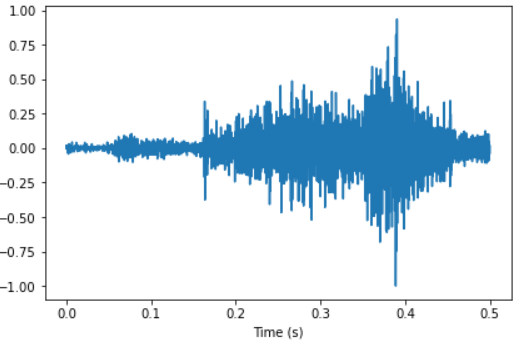
\includegraphics[width=\textwidth]{spectr_filter.png}
                \caption{Отфильтрованный спектр}
                \label{fig:spectr_filter}
            \end{figure}
            
            После всего этого переводим полученный спектр обратно в аудио:
            
            \begin{figure}[H]
                \centering
                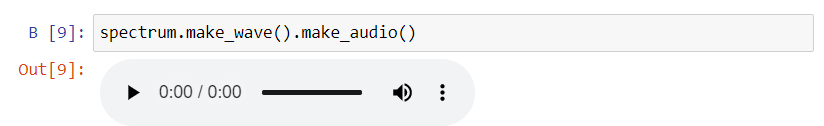
\includegraphics[width=\textwidth]{translate.png}
                \caption{Перевод спектра в аудио}
                \label{fig:spectr_translate}
            \end{figure}
            
            По результатам выполнеиня данного пункта можно сделать вывод, что полученный звук похож на оригинальный, но более приглушен, будто источник теперь находится в другой комнате
            
    \newpage
        \section{Часть №3: Комбинирование}
            В третьем пункте первой лабораторной работы нам необходимо создать сложный сигнал из объектов \texttt{SinSignal} и \texttt{CosSignal} суммируя их. Также следует обработать полученный сигнал для получения волный, прослушать его, вычислить для него  \texttt{Spectrum} и после вывести на экран.
            Для выполнения задания я взял синусоидальный канал с частотой \texttt{755 Hz} и косинусоидальный канал с частотой \texttt{400 Hz}:
            
\begin{lstlisting}[language=Python, caption= Создание каналов]
    from thinkdsp import CosSignal, SinSignal

    cos_sig = CosSignal(freq=400, amp=1.0)
    sin_sig = SinSignal(freq=755, amp=0.5)

    cos_sig.plot()
    decorate(xlabel='Time (s)')

    sin_sig.plot()
    decorate(xlabel='Time (s)')
\end{lstlisting}
            
            В результате получаем такой вывод на экран:
            \begin{figure}[H]
                \centering
                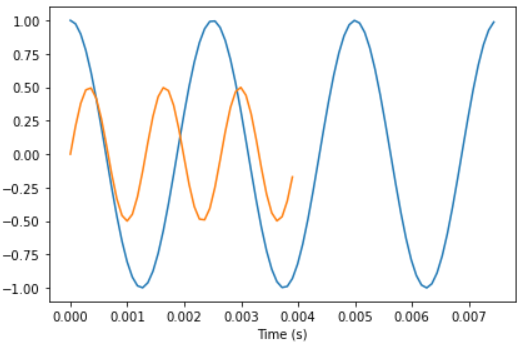
\includegraphics[width=\textwidth]{spectr_out.png}
                \caption{Вывод спектров}
                \label{fig:spectr_out}
            \end{figure}
            
            Теперь просуммируем эти два канала и выведем полученный суммирующий сигнал:
            
\begin{lstlisting}[language=Python, caption= Суммирование каналов]
    signal = cos_sig + sin_sig
    signal.plot()
    decorate(xlabel='Time (s)')
\end{lstlisting}
            
            \begin{figure}[H]
                \centering
                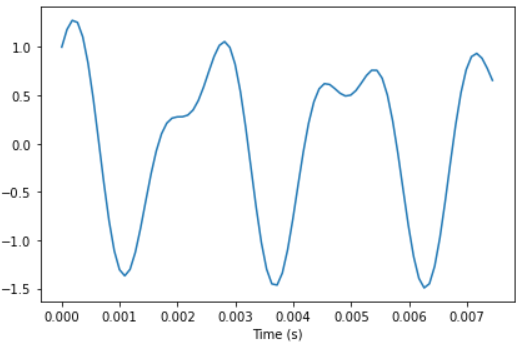
\includegraphics[width=\textwidth]{spectr_sum.png}
                \caption{Суммирование каналов}
                \label{fig:spectr_sum}
            \end{figure}
            
            После этого получим аудио из суммирующего канала
            
             \begin{figure}[H]
                \centering
                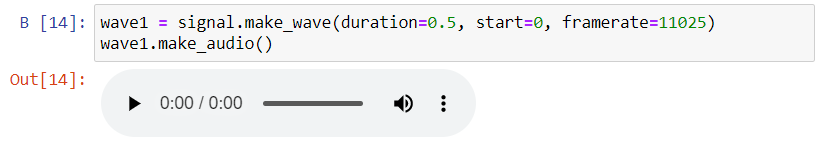
\includegraphics[width=\textwidth]{spectr_sum_audio.png}
                \caption{Получение аудио из сумирующего канала}
                \label{fig:spectr_sum_audio}
            \end{figure}
            
            Наконец, получим спектр из полученного сигнала:

\begin{lstlisting}[language=Python, caption= Получение спектра]
    spectrum = wave1.make_spectrum()
    spectrum.plot(high=1000)
    decorate(xlabel='Frequency (Hz)')
\end{lstlisting}
            
            \begin{figure}[H]
                \centering
                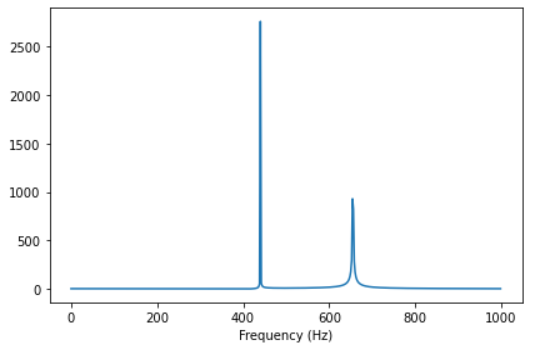
\includegraphics[width=\textwidth]{spectr_sum_result.png}
                \caption{Полученный спектр}
                \label{fig:spectr_sum_result}
            \end{figure}
            
            Добавим к полученному сигналу синусоидальный сигнал с частотой \texttt{450 Hz} ипереведем в аудио:
            
            \begin{figure}[H]
                \centering
                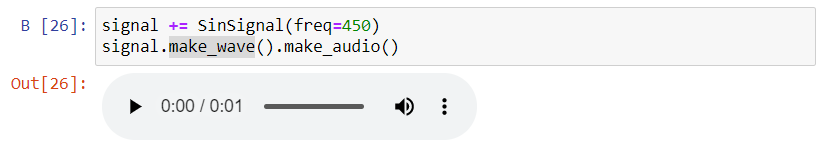
\includegraphics[width=\textwidth]{spectr_sum_add.png}
                \caption{Добавление к сигналу и перевод в аудио}
                \label{fig:spectr_sum_add}
            \end{figure}
            
            После всего этого нам остается только получить спектр из сигнала и вывести все на экран:
            
\begin{lstlisting}[language=Python, caption= Получение спектра и вывод на экран]
    wave2 = signal.make_wave()
    wave2.apodize
    spectrum2 = wave2.make_spectrum()
    spectrum2.plot(high=1000)
    decorate(xlabel='Frequency (Hz)')
\end{lstlisting}
            
            \begin{figure}[H]
                \centering
                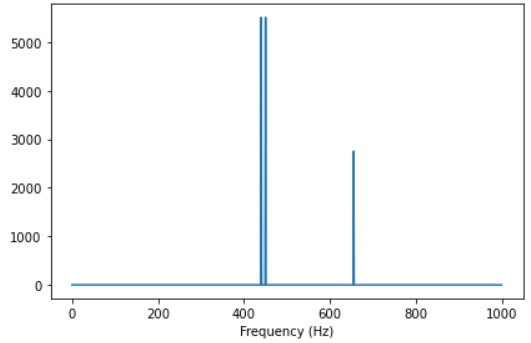
\includegraphics[width=\textwidth]{spectr_sum_add_result.png}
                \caption{Полученный спектр}
                \label{fig:spectr_sum_add_result}
            \end{figure}
            
            По результатам выполнения данного пункта можно сделать вывод, что полученный в самом конце звук теперь звучит громче и появились колебания, теперь этот звук достаточно тяжело слушать.
            
    \newpage
        \section{Часть №4: Растяжение}
            В четвертом пункте первой лабораторной работы нам необходимо реализовать функцию \texttt{stretch}, которая принимает сигнал и коэффициент изменения, после чего в зависимости от коэффициента либо замедляет, либо ускоряет сигнал посредством изменения \texttt{ts} и \texttt{framerate}.
            
            Перейдем к выполнению данного пункта. Сначала напишем саму функцию \texttt{stretch}:
            
\begin{lstlisting}[language=Python, caption= Функция \texttt{stretch}]
    def stretch(wave, factor):
    wave.ts *= factor
    wave.framerate /= factor
\end{lstlisting}
            
            После этого вызовем эту функцию, подав нашу оригинальную аудиодорожку и коэффициент изменения равный 0.4, затем получим аудиодорожку:
            
            \begin{figure}[H]
                \centering
                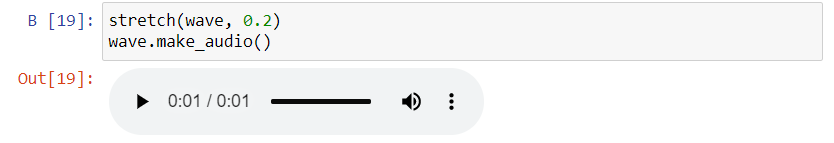
\includegraphics[width=\textwidth]{stretch_audio.png}
                \caption{Полученная в результате вызова функции \texttt{stretch} аудиодорожка}
                \label{fig:stretch_audio}
            \end{figure}
            
            Затем вызовем отображение спектра полученной дорожки на экран:
            
\begin{lstlisting}[language=Python, caption= Вывод на экран полученной после вызова функции \texttt{stretch} аудиодорожки]
    wave.plot()
    decorate(xlabel='Time (s)')
\end{lstlisting}
            
            \begin{figure}[H]
                \centering
                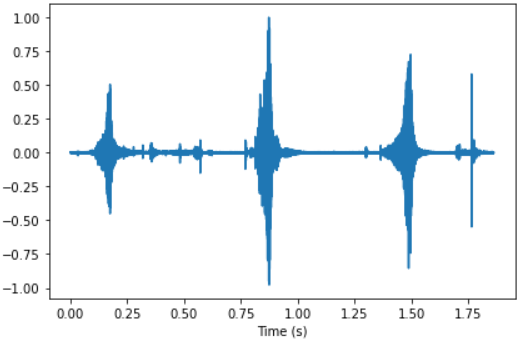
\includegraphics[width=\textwidth]{stretch_audio_result.png}
                \caption{Полученная в результате вызова функции \texttt{stretch} аудиодорожка}
                \label{fig:stretch_audio_result}
            \end{figure}
            
            По результатам выполнения данного пункта можно сделать вывод, что полученная функция \texttt{stretch} действительно замедляет и ускоряет полученный сигнал.
    
    \newpage
        \section{Выводы}
            В ходе выполнения лабораторной работы мы изучили способы работы с сигналами и возможности их обработки, фильтрации и воспроизведения с помощью библиотеки Python. Кроме того мы получили сведения об основных понятиях и навыки работы с сигналами, а также реализовали и проверели функцию для преобразования полученного сигнала. 
    
\end{document}
